% This template found at: https://tex.stackexchange.com/questions/42602/software-requirements-specification-with-latex
% It was a relatively simple template provided by SE user "Yiannis Lazarides"
% whose page is here: https://tex.stackexchange.com/users/963/yiannis-lazarides

%The scrreprt is part of the KOMA-script bundle of packages that does some 
%Fancy-schmancy tweaks to the typography of the resulting document. You know, 
%the kind of stuff that editors and designers love!
\documentclass{scrreprt}

%apparently something is deprecated, but using this package fixes that problem.
\usepackage{scrhack} 

%For code listings
\usepackage{listings}

%I honestly don't know what this is here for. Apparently it addresses some 
%weird edge case having to do with underscores and hyphenation of words. We 
%Could probably do without this package, but perhaps it's required by another 
%package.
\usepackage{underscore}

%How to handle hyperlinks.
\usepackage[bookmarks=true]{hyperref}
\hypersetup{
    bookmarks=true,    % show bookmarks bar?
    pdftitle={Software Requirement Specification},    % title
    pdfauthor={Team Moon Moon},                     % author
    pdfsubject={TeX and LaTeX},                        % subject of the document
    pdfkeywords={TeX, LaTeX, graphics, images}, % list of keywords
    colorlinks=true,       % false: boxed links; true: colored links
    linkcolor=blue,       % color of internal links
    citecolor=black,       % color of links to bibliography
    filecolor=black,        % color of file links
    urlcolor=purple,        % color of external links
    linktoc=all            % all makes whole line a link. "page" -> only page#
}%

%graphics
  \usepackage[pdftex]{graphicx}

%We use these renews so that our enumerations get sublisted with numbers 
%rather than letters.
\renewcommand{\labelenumii}{\theenumii}
\renewcommand{\theenumii}{\theenumi.\arabic{enumii}.}

\def\myversion{0.1.0 }
\title{%
\flushright
\rule{16cm}{5pt}\vskip1cm
\Huge{SOFTWARE REQUIREMENTS\\ SPECIFICATION}\\
\vspace{2cm}
for\\
\vspace{2cm}
Online Postage Ordering System\\
\vspace{2cm}
\LARGE{Release 0.1.0\\}
\vspace{2cm}
\LARGE{Version \myversion approved\\}
\vspace{2cm}
Prepared by Team Moon Moon\\
\vfill
\rule{16cm}{5pt}
}

\date{}

\usepackage{hyperref}
\author{Team Moon Moon}

\begin{document}
\maketitle
\tableofcontents

\chapter*{Revision History}

\begin{enumerate}
\item Team Moon Moon Needs No Revisions.
\item Team Moon Moon Never Makes No Mistakes.
\item Correction. Team Moon Moon ``fails fast.'' Isn't that the new 
buzzword or buzzphrase?
\item The skeleton has been updated to reflect the actual requirements 
provided by Dr. Seaman.
\item It's all really coming together now.
\item Final Revision for Turn-In
\end{enumerate}

\chapter{Introduction}

\section{Purpose}

The purpose of this document is to present a detailed description of the
specifications and the requirements for a postage printing website. It will
explain the purpose and features of the system, the interfaces of the system,
what the system will do, the constraints under which it must operate, and how
the system will react to interactions. This document is intended for both the
stakeholders and the developers of the system.

\section{Project Scope and Product Features}

The objective of this project is to create and implement a website for printing
mailing labels containing USPS postage. The website will be used primarily by
registered users. The website will allow users to: 

\begin{itemize}
\item Create and maintain individual secured accounts
\item Buy/print postage labels
\item List postage purchase history
\item Check account balance
\item Calculate postage rates
\item Track packages
\item Request refunds
\item Check if an address is valid
\end{itemize}

\section{Defintions, Acronyms, and Abbreviations}

At this time, there are no specialized terms in need of definition.

\section{References}

IEEE. IEEE Std 830-1998 IEEE Recommended Practice for Software Requirements
Specifications. IEEE Computer Society, 1998.

\section{Overview}

The second section, the Overall Description, of this document gives an overview
of the products functionality. It describes the informal requirements and is
used to establish a context for the requirements specification in the third
section.

The third section, Requirements Specification, of this document is written
primarily for the developers. It describes details of product functionality. 

\chapter{Overall Description}

This chapter provides an overview of the software product from the perspective 
of the functions that the user is expected to have available to him.

\section{Product Perspective}

The overall idea is that the user may print pre-labelled postage from a
website. The website provides an address verification service, and is licensed
by the relevant governments to sell postage that the relevant governments’
postal services will honor. This makes obtaining and labelling postage much
quicker than by traditional means, wherein one had to drive to the post office
to obtain stamps, and had no way to verify the existence of any particular
address. As well, the user can either add credit to the website or purchase
postage on a one-off basis, and can access a record of all transactions made
with the website.

%\begin{figure}[H]
%\centering
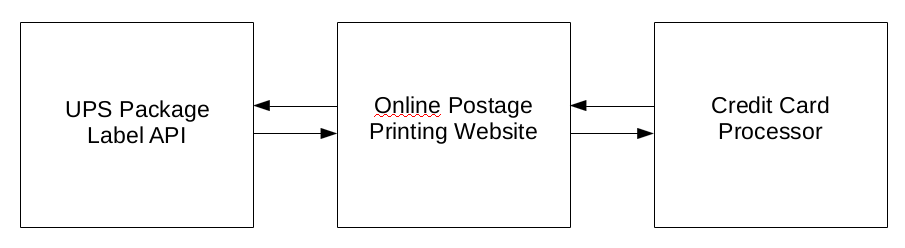
\includegraphics[scale=.4]{2-1-product-perspective.png}
%\label{sec_2_1}
%\end{figure}

\section{Product Functions}

The following subsections detail the various functions that the user of the 
software must be able to utilize.

\subsection{Create An Account}

The Create Account function shall allow a user to create a secure account. The
account will track the user’s full name, mailing address, email address, credit
card information, username and password, and the purchase history for up to two
years.

\subsection{Print Postage}

The Print Postage function shall allow the user to print postage that has been 
purchased, \emph{directly to a printer and NOT to a file.} The postage label 
will be provided upon successfully calling the UPS API, which will return an 
image suitable for printing. 

\subsection{Buy Postage}

The Buy Postage function shall allow the user to purchase postage, using
available credit on their account. Upon a successful print, the user's account 
balance is appropriately debited.

\subsection{List Postage Transactions}

The List Postage Transactions function shall allow the user to view a list of
all of the postage labels that they have printed, including the information
printed on the label, over the past two years.

\subsection{Get Postage Balance}

The Get Postage Balance function shall allow the user to obtain their current
amount in their postage buying account.

\subsection{Calculate Postage}

The Calculate Postage function shall allow the user to enter a name, address,
package type, mail class, and weight. The user shall then be able to see a
calculated postage amount to ship their package.

\subsection{Track/Confirm Package}

The track/confirm package function shall allow users to enter in a tracking
number to see the status of their package. The status of the package will be
received from USPS  and displayed to the user. 

\subsection{Login/Password Reset}

The login function shall allow account members to enter their username and
password.  When verified with the system database, users will be able to access
restricted functions. The login function shall provide users an option to
reset their password. 

\subsection{Refund Request}

The Refund Request function shall allow the user to enter a date and to select
from a list any postage purchase made on that date that they wish to refund as
long as it is not older than ten days old.

\subsection{Validate Address}

The Validate Address function shall allow the user to enter an address to
verify its validity.

\subsection{Logout}

The logout function shall allow the account user to exit out of their account
for security.

\section{User Characteristics}

Users are expected to be Internet literate and be able to navigate in a
website.

\section{Constraints}

While the system does not have any restricting hardware or software
constraints, the system does have some constraints on the user which are
described in the 2.3 User Characteristics part of this document.

\section{Assumptions and Dependencies}

It is assumed that the end user: 

\begin{itemize}
\item Has an Internet connection. 
\item Has a web browser able to display the website.
\item Has a printer.
\end{itemize}

\chapter{Specific Requirements}

\section{External Interface Requirements}

This section details any significant interfaces that the Online 
Postage Printing Website will encounter.

\subsection{System Interfaces}

There are two main system interfaces:

\begin{enumerate}
\item The online credit card processing system. The website will 
access this system via an API to charge cards.
\item The UPS postage label API. The website will make several 
queries to the UPS' APIs in order to calculate shipping cost and 
retrieve labels.
\end{enumerate}

\subsection{User Interfaces}

IN-PROGRESS.

\subsection{Hardware Interfaces}

IN-PROGRESS.

\subsection{Software Interfaces}

IN-PROGRESS.

\subsection{Communication Interfaces}

IN-PROGRESS.

\section{Functional Requirements}

The following subsections describe, in detail, the requirements for 
the system in order to provide each function described in section 
2.2.

\subsection{Create an Account}

\begin{enumerate}
\item The system requires, from the user, the following information: Full Name,
Mailing Address, Email Address, Credit Card information, a unique username, and
a password.
\begin{enumerate}
\item Invalid data is prevented from being entered.
\item The username and password should meet the specified criteria [TBD].
\item If the selected username and password do not meet the criteria, the
system shall ask the user to reenter a new username and password.
\end{enumerate}
\item All provided information, entered by the user, should be stored in the
system.
\end{enumerate}

\subsection{Print Postage}

The system shall...

\begin{enumerate}
\item First, ensure...
\begin{enumerate}
\item that there is a valid, logged-in user requesting the postage.
\item that the user is authorized to print the postage.
\item that the user's printer is available and functional.
\end{enumerate}
\item Then, prompt the user to confirm the printing of the postage, showing
current and subsequent account balances as necessary.
\item Then, once confirmation from the user is obtained, generate the postage
on a special page, devoid of any other content, that the user may print. Ensure
that the user is unable to print to a file.
\item Finally, upon detection of the completed print job, return the user to
the ``account status'' page, where the successful print job is displayed in the
list of transactions.
\end{enumerate}

\subsection{Buy Postage}

The system shall...

\begin{enumerate}
\item First, ensure
\begin{enumerate}
\item that there is a valid, logged-in user requesting to buy postage.
Otherwise, redirect to the Log In function.
\end{enumerate}
\item Then, provide the user with options of what sort of postage to purchase.
\item Then, upon the user selecting a package, query for the quantity of
postage to purchase.
\item Then, upon obtaining the quantity, calculate the total cost and prompt
the user for a purchase method, either through account credit or through a
one-time payment.
\begin{enumerate}
\item If the user wishes to utilize account credit, ensure that sufficient
credit is available to cover the total cost. If there is enough credit, proceed
to step 5. Otherwise, prompt user to add credit to their account or perform a
one-time purchase.
\item If the user wishes to purchase through a one-time payment, proceed to
step 6.
\end{enumerate}
\item Upon confirming that enough credit is available, request the address for
the postage to be delivered to and pass this address to the validate address
function. If the validate address function confirms the validity of the
address, proceed to step 8. Otherwise, prompt again for a valid address.
\item Upon confirming that the user wishes to make a one-time payment, request
the credit card information, either stored on the account or provided manually.
Proceed to step 7.
\item Upon confirmation of the one-time payment details, request an address for
delivery. Pass the address to the address verification function. If the address
is valid, proceed to step 8. Otherwise, request a valid address.
\item Then, confirm the transaction details: amount, price, shipping
destination.
\item Upon confirmation from the user, enter the transaction into the
transaction ledger, schedule the postage for printing, and proceed to the Print
Postage function.
\end{enumerate}

\subsection{List Postage Transactions}

The system shall...

\begin{enumerate}
\item First, ensure that there is a valid, logged-in user requesting to view
the Postage Transactions.
\item Then, provide a method for the user to select a start
date and then an end date for which they would like to view the postage
transactions.
\item Then, query the database, using the selected dates as
the requirements, and will list any and all Postage Transactions that fall
between the specified dates in descending order.
\end{enumerate}

\subsection{Get Postage Balance}

The system shall...

\begin{enumerate}
\item First, ensure...
\begin{enumerate}
\item that there is a valid, logged-in user requesting the postage balance.
\item that the user is authorized to view the postage balance.
\end{enumerate}
\item Then, find user account, and display postage balance in order for the
user to see.
\end{enumerate}

\subsection{Calculate Postage}

The system shall...

\begin{enumerate}
\item First, ensure that there is a valid, logged-in user requesting the
postage balance.  
\item Then, provide a method for the user to enter a Name,Address,Packaging
type, mail class, and weight.
\item Then, calculate estimated shipping cost for the users package.
\item Finally, upon completion of calculation, display the estimated shipping
costs.  
\end{enumerate}

\subsection{Track/Confirm Package}

The system shall...

\begin{enumerate}
\item allow the user to enter in a tracking number.
\item check the tracking number with the system database.
\begin{enumerate}
\item if valid, display the current tracking information for the user to
access.
\item if invalid, inform the user that the tracking number is not in the system
database. The user may enter a tracking number or the user may cancel. 
\end{enumerate}
\end{enumerate}

\subsection{Login/Password Reset}

The system shall...

\begin{enumerate}
\item require a username and password from the user.
\item verify the username and password with the system database.
\begin{enumerate}
\item If valid, the user will be granted access to the following functions:
\item If the username is not located within the system database, the system
shall inform the user that their username is invalid. The user may enter a
different username or the user may cancel.
\item If password is not valid for the username entered, inform the user that
the password is invalid. The user many enter a different password or the user
may cancel 
\end{enumerate}
\item allow the user to request a password from the system to be emailed to the
registered user.
\begin{enumerate}
\item The user can request a password from the system, provided the user gives
the system a valid username from the system database.
\begin{enumerate}
\item If the username is not within the database, inform the user that their
username is invalid. The user may enter a different username of the user may
cancel.
\end{enumerate}
\item The system shall randomize a password and send to the users accounts
email in the system database.
\end{enumerate}
\end{enumerate}

\subsection{Refund Request}

The system shall...

\begin{enumerate}
\item First, ensure that there is a valid, logged-in user requesting to access
the Refund Request function
\item Then, provide a method for the user to enter a date.
\item Then, query the database for any postage transactions
made on that date.
\item Then, display a list of any and all postage transactions
made on that date in descending order.
\begin{enumerate}
\item mark those transactions that are eligible for refund by
determining which transactions fall within the ten day window.
\end{enumerate}
\item Then, provide a method for the user to select an
eligible transaction to be invalidated and refunded.
\item Then, provide a method for the user to confirm the
selection.
\begin{enumerate}
\item mark the selected transaction as invalid.
\item adjust the user’s Postage Balance to reflect the
refunded amount.
\end{enumerate}
\end{enumerate}

\subsection{Validate Address}

The system shall...

\begin{enumerate}
\item First, provide a method for the user to enter an address to validate.
\item Then, query a database of addresses in an attempt to
validate the entered address.
\begin{enumerate}
\item If the address is not found in the database, attempt to find an address
that is similar to the entered address.
\item If a similar address is found, notify the user that the entered address
is not found and display the similar address and ask the user to confirm the
new address.
\item If no similar address is found, notify the user that the entered address
is invalid and prompt them to enter a new address.
\end{enumerate}
\end{enumerate}

\subsection{Logout}

The system shall...

\begin{enumerate}
\item immediately disable access to functions that require a registered user.
\end{enumerate}

\section{Performance Requirements}

1500 people should be able to use web application simultaneously. System
login/logout shall take less than eight seconds. Requests to Print Postage
should be processed within 10 seconds. All other requests should be processed
within 5 seconds.

\section{Logical Structure of the Data}

IN-PROGRESS. Assigned to Preston Maness (me). I'm still working on a good 
way to diagram everything.

\section{Design Constraints}

Constraints for the postage printing website include

\begin{itemize}
\item Able to support PC, Mac platforms.
\item System logs out user after ten minutes of inactivity.
\item System supports all web browsers.
\end{itemize}

\section{Software System Attributes}

The requirements in this section specify the required reliability,
availability, security and maintainability of the software system.

\subsection{Reliability}

For the system to be reliable it will require a stable Internet connection. If
service goes down, it should be restored within 20 minutes. The average failure
rate should be less than 4\% of all transactions.

\subsection{Availability}

The system should not be unavailable for more than 30 minutes within a 24 hour
period, on average.

\subsection{Security}

Users access should be limited to their personal information only. Purchases
should be handled through a secure server to ensure the protection of the
user’s credit card and personal information.

\subsection{Maintainability}

Any updates or fixes shall be able to be made on server-side only, without any
requirements of the user.

\subsection{Portability}

Nothing required.

% add other chapters and sections to suit
\end{document}
